\documentclass[11pt]{article}
\usepackage{amsmath,amssymb,amsthm,amsfonts,hyperref, enumitem, tikz}

\title{Puck Predictions: Unraveling the NHL Game Forecasting Riddle}
\author{Jason Vasquez \and Dylan Skinner \and Jeff Hansen \and Benjamin McMullin}

\begin{document}

\maketitle

\begin{abstract}
    The goal of this project is simple: predict the outcomes of NHL games from any given state.
    As simple as the problem statement is, however, the solution is not so straightforward.
    To solve this problem, we will use a variety of machine learning techniques, including logistic regression,
    XGBoost, and ARIMA models. Additionally, we utilize a form of MCMC to simulate the outcomes of games from any given
    state. Our hypothesis is that we will be able to successfully predict the outcomes of NHL games with a high degree of accuracy
    using these tools.
\end{abstract}

\section{Problem Statement and Motivation}
% Your content for this section goes here
In the world of sports analytics, predicting the outcomes of games is a common and challenging problem, with live win predictions adding
an extra layer of complexity. For most sports, there are a plethora of widely accepted—yet hidden—predictive models and methods that are used to
predict games. In addition to this, most sports have easily accessible statistics and graphics that give current win probabilities for any live game.

Hockey, however, is a different story. While there are some methods used to predict the outcome of National Hockey League (NHL) games, these models
typically belong to sport books and their nuances are not publicly disclosed. Additionally, hockey analytics is not as
developed as it is in other sports, such as basketball or baseball. This lack of model transparency and public interest in hockey analytics
makes predicting the outcomes of NHL games a challenging problem. That is where this project comes in. The goal of this project is simple: predict
the outcomes of NHL games and provide a live win probability for any given game state.

Despite the simplicity of the problem statement, as mentioned, the solution is not so straightforward. The NHL provides fast-paced games with many events
occuring in quick succession. Our goal is to sift through the data points and identify key features that will allow us to predict the outcome of a game and
ignore other features that exist as seeming proxy noise.

Our motivation for this project exists strictly as fans of the sport and as data scientists. Our model is not intended to be used for gambling or any other
nefarious purposes—any use of this model for such purposes is a misuse of our work.

\section{Data}
% Your content for this section goes here
Our data came from the hockeyR Github repository\cite{hockeyR-data}. This repository contains an abundance of data about every NHL game
that has occured since the 2010-11 season. This data includes information about the events that transpire in a game (hits, shots, goals, etc.),
which teams are playing, who is on the ice, and the final score of the game. The data is stored in a series of {\tt .csv.gz} files, allowing for
easy access and manipulation.

Each game in a season is given a unique identifier ({\tt game\_id}), which is constant across all events in a game. Every event that occurs in a game
will be stored in the {\tt event\_type} column. There are 17 unique event types, including things such as game start, faceoff, shot, hit, and goal.
Most of these event types are not relevant to our analysis, so we remove them from the dataset. After removing the unnecessary events, we are left with
nine events: blocked shot, faceoff, giveaway, goal, hit, missed shot, penalty, shot, and takeaway. These events are attributed to the
team and player that performs the event. We only take into consideration the team that performs the event and discard the player information.

The data also contains information about when the event occured. This appears in a variaty of formats, but we only
use the {\tt game\_time\_remaining} column. {\tt game\_time\_remaining} starts
at 3600 (60 minutes) and counts down to 0. If the game goes into extra time, i.e., it is tied after 60 minutes, {\tt game\_time\_remaining} will
be a negative value.

We found that our data did not contain any missing values that was not easily explainable. For example, if a game is starting, there will be no
events for penalties, which will result in a {\tt NaN} value in the penalties column. Additionally, any data that was confusing or not easily explainable
(for example the home team having 7 players on the ice and the away team having 5), was manually verified by watching a clip of the game where
the event occured to make sure the event was recorded correctly. We did not find any incorrectly recorded events, so we 
did not remove any strange events from out dataset.

\section{Methods}

\subsection{Bayesian Network}
We first used a Bayesian Network to establish a benchmark for probability using several key features.

Bayesian networks are probabilistic graphical models that represent probabilistic relationships among a set of variables using a directed acyclic graph (DAG). 
In a Bayesian network, nodes represent random variables, and directed edges between nodes represent probabilistic dependencies between the variables. Each node in the graph is associated with a conditional probability distribution that quantifies the probability of that variable given its parent variables in the graph.

For our purposes, we predefined the structure of the network, and used the data to calculate the conditional probabilities for each node. We then used the network to calculate the probability of a team winning given the current state of the game.

The computational complexity of Bayesian Network inference is high, with exact inference being an NP-hard problem TODO CITE. 
Using the python package pgmpy, we originally tried to fit a network with all 26 of our features, but our computational resources failed to fit this network.
Then, to get a baseline for our future predictions, we simply fitted the model with the base features of home goals, away goals, home shots, away shots, home blocked shots, and away blocked shots. 
These features were chosen as priors because of our opinion that they are the most important to the game, based upon our knowledge of hockey.


(Basic graph to test)

\begin{center}
    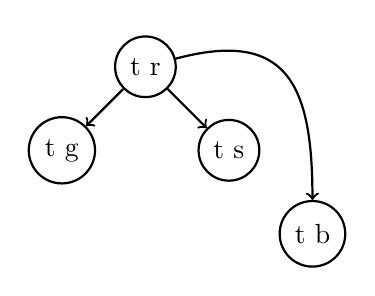
\begin{tikzpicture}[node distance={15mm}, thick, main/.style = {draw, circle}]
        \node[main] (1) {t r}; 
        \node[main] (2) [below left of=1] {t g};
        \node[main] (3) [below right of=1] {t s};
        \node[main] (4) [below right of=3] {t b};

        \draw[->] (1) -- (2);
        \draw[->] (1) -- (3);
        \draw[->] (1) to [out=15,in=90,looseness=1.5] (4);

    \end{tikzpicture} 
\end{center}

\subsection{t-SNE, UMAP, and PCA}

\subsection{Regression and XGBoost}

\subsection{MCMC Game Simulation}

\section{Results}
% Your content for this section goes here

\section{Analysis}
% Your content for this section goes here

\section{Ethical Considerations}
Predicting win percentages or outcomes in hockey games, like any sport, raises several ethical considerations. Here are some key points we want to address:

\begin{itemize}[label=\textbullet]
\item \textbf{Gambling and Addiction}:
Our win percentages and predictions might be used by those who wish to gamble, which could lead to addiction and financial harm, especially if undue trust in placed in these methods. Any publication of these methods or predictions would be accompanied by promoting healthy and responsible gambling practices.
    
\item \textbf{Fairness and Integrity of the Game}:
Sometimes, coaches and players becoming aware of their chance of winning can affect how the game is played, potentially harming the integrity of the sport. We must be careful to not provide an unfair advantage to any team or player.
Inaccurate predictions could lead a team to believe that the game is out of reach when it isn't, and we want to avoid that.
            
\end{itemize}

Overall, our predictions, like any, should not be considered declarative for gambling or performance purposes, but are rather an interesting exposition into the complexity of sporting events.


\section{Conclusions}
% Your content for this section goes here

% Bibliography
\bibliographystyle{plain}
\bibliography{references} % Replace 'references' with the name of your .bib file

\end{document}

